% Anexo técnico del Reto AgroCebada FIRA 2026. Máximo 4 cuartillas de contenido, más las referencias, con la tabla de
% ID y rendimiento predicho.
% Sigue la plantilla oficial de IEEE para conferencias (bare_conf.tex de IEEEtran v1.8b).
% cite.sty e IEEEtran.cls van en esta carpeta porque no vienen en el TeX Live instalado.
% Compilar desde reporte/entrega (dos veces):
%   xelatex -interaction=nonstopmode anexo_tecnico.tex && xelatex -interaction=nonstopmode anexo_tecnico.tex
% Las referencias van al final del mismo archivo (referencias.tex, que genera plataforma.py).
\documentclass[conference,letterpaper]{IEEEtran}
\usepackage{fontspec}
\setmainfont{TeX Gyre Termes}
\usepackage{polyglossia}
\setdefaultlanguage{spanish}
\usepackage{cite}
\usepackage{amsmath,amssymb}
\usepackage{graphicx}
\usepackage[caption=false,font=footnotesize]{subfig}
\usepackage{booktabs}
\usepackage{array}
\usepackage{xcolor}
\usepackage{etoolbox}
\usepackage{hyperref}
\hypersetup{colorlinks=true,linkcolor=black,citecolor=black,urlcolor=blue!50!black}
\graphicspath{{figuras/}}
\gappto\captionsspanish{\renewcommand{\figurename}{Fig.}\renewcommand{\tablename}{Tabla}}
\renewcommand{\IEEEkeywordsname}{Palabras clave}
% Menos espacio alrededor de las figuras para caber en 4 cuartillas.
\setlength{\textfloatsep}{9pt plus 2pt minus 2pt}
\setlength{\dbltextfloatsep}{8pt plus 2pt minus 2pt}
\setlength{\intextsep}{9pt plus 2pt minus 1pt}
\setlength{\abovecaptionskip}{4pt}
\renewcommand{\dbltopfraction}{0.8}
\renewcommand{\topfraction}{0.85}
\renewcommand{\textfraction}{0.1}

\begin{document}

\title{Anexo técnico. Rendimiento de cebada de temporal\\con régimen de registro y rezago espacial}

\author{\IEEEauthorblockN{José Alán Pomares Valdés, Vicente Josimar López Martínez, Luis Emmanuel Ramiro Luna\\y Luis Gustavo Olivares Soto (asesor)}
\IEEEauthorblockA{Facultad de Ciencias de la Computación, Benemérita Universidad Autónoma de Puebla\\Puebla, México, 
pv202351433@alm.buap.mx}}

\maketitle


\begin{abstract}
Buscamos predecir el rendimiento de 59 parcelas de cebada de temporal a partir de 138 con rendimiento conocido. Vimos
que cada municipio registra el rendimiento de una de dos formas, con medias muy distintas, y que esa diferencia pesa
más que cualquier variable satelital, climática o topográfica. Sobre ella construimos el modelo de parcelas, y como
solo sirve cerca de parcelas con rendimiento conocido, agregamos un modelo municipal con datos públicos de 2003 a 2025
para toda la región. El primero es un proceso gaussiano~\cite{rasmussen2006} con el régimen de registro y el
rendimiento de las parcelas vecinas, con raíz del error cuadrático medio (RMSE)~\cite{chai2014} esperada de 0.46 a
0.49\,t/ha. El segundo es una regresión sobre la temperatura máxima de verano con un kriging~\cite{oliver2014} de sus
errores, con RMSE de 0.44\,t/ha en municipios sin datos cercanos. La Tabla~\ref{tab:predicciones} lista el ID y el rendimiento predicho de las 59 parcelas. El detalle está
en los reportes del equipo~\cite{doc_contexto,doc_modelo,doc_generalizable} y el código en su repositorio~\cite{repo}.
\end{abstract}

\begin{IEEEkeywords}
rendimiento de cebada, régimen de registro, rezago espacial, proceso gaussiano, kriging, datos públicos, crédito agrícola.
\end{IEEEkeywords}

% La tabla obligatoria se define aquí para que quede arriba de la página 2.
% Tabla de las 59 predicciones, tomada de outputs/predicciones_finales.csv.
\begin{table*}[!t]
\centering
\caption{Rendimiento predicho (Pred.), intervalo p10 a p90 (t/ha) y probabilidad de rendimiento menor que 2.5\,t/ha de las 59 parcelas. R es el régimen y $P$ la probabilidad.}
\label{tab:predicciones}
\scriptsize
\setlength{\tabcolsep}{3.5pt}
\begin{tabular}{@{}llcrrrr@{\hspace{1.6em}}llcrrrr@{}}
\toprule
ID & Municipio & R & Pred. & p10 & p90 & $P$ & ID & Municipio & R & Pred. & p10 & p90 & $P$ \\
\midrule
AGC\_003 & Singuilucan & B & 3.66 & 3.11 & 4.14 & 0.000 & AGC\_107 & Almoloya & A & 4.54 & 4.03 & 5.12 & 0.001 \\
AGC\_011 & Chignahuapan & A & 4.54 & 4.03 & 5.11 & 0.001 & AGC\_113 & Singuilucan & B & 3.25 & 2.70 & 3.73 & 0.031 \\
AGC\_016 & Chignahuapan & A & 4.57 & 4.06 & 5.14 & 0.001 & AGC\_116 & Chignahuapan & A & 4.54 & 4.03 & 5.12 & 0.001 \\
AGC\_025 & Calpulalpan & B & 2.98 & 2.43 & 3.46 & 0.225 & AGC\_118 & Singuilucan & B & 3.02 & 2.47 & 3.50 & 0.196 \\
AGC\_027 & Calpulalpan & B & 3.02 & 2.47 & 3.50 & 0.196 & AGC\_120 & Nanacamilpa & B & 3.02 & 2.47 & 3.50 & 0.196 \\
AGC\_028 & Chignahuapan & A & 4.54 & 4.03 & 5.12 & 0.001 & AGC\_126 & Chignahuapan & A & 4.57 & 4.06 & 5.14 & 0.001 \\
AGC\_029 & Calpulalpan & B & 3.02 & 2.47 & 3.50 & 0.196 & AGC\_128 & Almoloya & A & 4.56 & 4.05 & 5.13 & 0.001 \\
AGC\_030 & Singuilucan & B & 3.02 & 2.47 & 3.50 & 0.196 & AGC\_129 & Singuilucan & B & 3.02 & 2.47 & 3.50 & 0.196 \\
AGC\_031 & Chignahuapan & A & 3.88 & 3.37 & 4.45 & 0.023 & AGC\_130 & Cuautepec & A & 4.54 & 4.03 & 5.11 & 0.001 \\
AGC\_036 & Chignahuapan & A & 4.55 & 4.04 & 5.12 & 0.001 & AGC\_136 & Chignahuapan & A & 4.57 & 4.06 & 5.14 & 0.001 \\
AGC\_039 & Calpulalpan & B & 3.02 & 2.47 & 3.50 & 0.196 & AGC\_142 & Chignahuapan & A & 4.56 & 4.04 & 5.13 & 0.001 \\
AGC\_042 & Singuilucan & B & 3.25 & 2.70 & 3.73 & 0.031 & AGC\_143 & Chignahuapan & A & 4.58 & 4.07 & 5.15 & 0.001 \\
AGC\_043 & Chignahuapan & A & 4.57 & 4.06 & 5.14 & 0.001 & AGC\_147 & Calpulalpan & B & 3.02 & 2.47 & 3.50 & 0.196 \\
AGC\_050 & Calpulalpan & B & 3.02 & 2.47 & 3.50 & 0.196 & AGC\_149 & Cuautepec & A & 4.54 & 4.03 & 5.12 & 0.001 \\
AGC\_052 & Cuautepec & A & 4.56 & 4.05 & 5.14 & 0.001 & AGC\_153 & Chignahuapan & A & 4.54 & 4.03 & 5.11 & 0.001 \\
AGC\_061 & Calpulalpan & B & 3.02 & 2.47 & 3.50 & 0.196 & AGC\_154 & Chignahuapan & A & 4.58 & 4.07 & 5.15 & 0.001 \\
AGC\_063 & Chignahuapan & A & 4.54 & 4.03 & 5.11 & 0.001 & AGC\_156 & Singuilucan & B & 3.02 & 2.47 & 3.50 & 0.196 \\
AGC\_065 & Almoloya & A & 4.54 & 4.03 & 5.11 & 0.001 & AGC\_158 & Chignahuapan & A & 4.50 & 3.99 & 5.07 & 0.001 \\
AGC\_071 & Calpulalpan & B & 3.08 & 2.53 & 3.56 & 0.049 & AGC\_173 & Calpulalpan & B & 3.02 & 2.47 & 3.50 & 0.196 \\
AGC\_075 & Calpulalpan & B & 2.98 & 2.43 & 3.46 & 0.225 & AGC\_174 & Cuautepec & A & 4.54 & 4.03 & 5.11 & 0.001 \\
AGC\_076 & Chignahuapan & A & 4.54 & 4.03 & 5.11 & 0.001 & AGC\_175 & Chignahuapan & A & 4.58 & 4.07 & 5.15 & 0.001 \\
AGC\_082 & Almoloya & A & 4.54 & 4.03 & 5.11 & 0.001 & AGC\_177 & Chignahuapan & A & 3.72 & 3.21 & 4.29 & 0.024 \\
AGC\_085 & Chignahuapan & A & 3.72 & 3.21 & 4.29 & 0.024 & AGC\_182 & Chignahuapan & A & 4.58 & 4.07 & 5.15 & 0.001 \\
AGC\_086 & Calpulalpan & B & 3.02 & 2.47 & 3.50 & 0.196 & AGC\_183 & Calpulalpan & B & 3.02 & 2.47 & 3.50 & 0.196 \\
AGC\_087 & Calpulalpan & B & 2.75 & 2.20 & 3.23 & 0.235 & AGC\_186 & Chignahuapan & A & 4.54 & 4.03 & 5.11 & 0.001 \\
AGC\_088 & Chignahuapan & A & 4.45 & 3.94 & 5.02 & 0.002 & AGC\_188 & Chignahuapan & A & 4.58 & 4.07 & 5.15 & 0.001 \\
AGC\_091 & Chignahuapan & A & 4.55 & 4.04 & 5.13 & 0.001 & AGC\_190 & Chignahuapan & A & 4.47 & 3.95 & 5.04 & 0.002 \\
AGC\_093 & Calpulalpan & B & 2.98 & 2.43 & 3.46 & 0.225 & AGC\_191 & Chignahuapan & A & 4.56 & 4.04 & 5.13 & 0.001 \\
AGC\_094 & Chignahuapan & A & 4.56 & 4.05 & 5.13 & 0.001 & AGC\_192 & Chignahuapan & A & 4.54 & 4.03 & 5.11 & 0.001 \\
AGC\_095 & Chignahuapan & A & 4.58 & 4.07 & 5.15 & 0.001 & \multicolumn{7}{c}{} \\
\bottomrule
\end{tabular}
\end{table*}


\section{Dos formas de registrar el rendimiento}

\begin{figure}[!b]
\centering
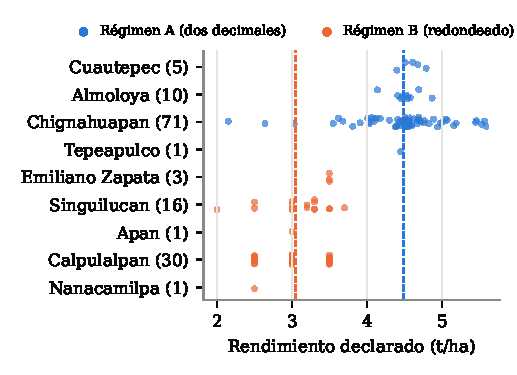
\includegraphics[width=0.66\columnwidth]{f1_regimenes}
\caption{Rendimiento de las 138 parcelas de entrenamiento por municipio. Cada municipio cae en un solo régimen. Las
líneas punteadas son la media de cada régimen.}
\label{fig:regimenes}
\end{figure}

Cada municipio registra el rendimiento de una sola forma (Fig.~\ref{fig:regimenes}). En el régimen A los valores
tienen dos decimales y promedian 4.49\,t/ha. En el B tienen un decimal y promedian 3.05\,t/ha. La diferencia entre
medias, 1.4\,t/ha, es casi tres veces la desviación estándar dentro de cada régimen. Por eso el régimen es la primera
pieza del modelo. No sabemos si el rendimiento se midió distinto o solo se anotó distinto (Sección~VIII).


\textbf{El régimen supera a la media por municipio.} La media
por municipio se acerca a la del régimen en el esquema A, una validación cruzada~\cite{hastie2009} con 5 grupos
estratificados por municipio repetida 10 veces como la partición de FIRA. Cuando la validación deja fuera zonas
completas~\cite{roberts2017} (esquema B) sube a 0.955\,t/ha. El régimen se
asigna por municipio y las 59 parcelas de prueba están en municipios con entrenamiento.


\section{Modelo}


\textbf{Rezago espacial.} Parcelas cercanas tienden a rendir parecido~\cite{tobler1970}. El rezago de la parcela $i$ es un promedio por distancia
inversa~\cite{shepard1968}
\begin{equation}
\ell_i = \frac{\sum_{j\in\mathcal{N}_i} y_j / d_{ij}}{\sum_{j\in\mathcal{N}_i} 1 / d_{ij}},
\label{eq:rezago}
\end{equation}
donde $\mathcal{N}_i$ son hasta 10 parcelas de entrenamiento del mismo régimen a 400\,m o menos, $y_j$ su rendimiento y
$d_{ij}$ la distancia. Sin vecinos, $\ell_i$ es la media del régimen en el entrenamiento. La parcela evaluada nunca
entra en su propio rezago. Elegimos 400\,m porque es el radio con menor error (Fig.~\ref{fig:radio}), aunque es el único bajo la media por
régimen y por eso la ventaja es frágil. La validación anidada~\cite{varma2006} cobra esa elección
(Sección~\ref{sec:confiabilidad}).

\begin{figure}[!htb]
\centering
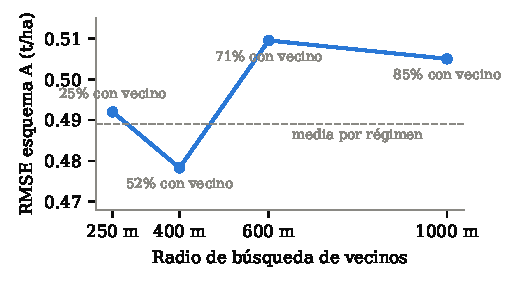
\includegraphics[width=0.60\columnwidth]{f3_radio}
\caption{RMSE según el radio de búsqueda de vecinos, con la fracción de parcelas que tiene al menos un vecino.}
\label{fig:radio}
\end{figure}



\textbf{Proceso gaussiano.} Las entradas son el régimen en dos columnas indicadoras y el rezago estandarizado. La
covarianza entre dos parcelas es
\begin{equation}
k(\mathbf{x},\mathbf{x}') = \sigma_f^2 \exp\!\left(-\frac{\lVert\mathbf{x}-\mathbf{x}'\rVert^2}{2\lambda^2}\right) +
\sigma_n^2\,\delta_{\mathbf{x}\mathbf{x}'},
\label{eq:kernel}
\end{equation}
donde $\lambda$ es la escala de parecido, $\sigma_f^2$ la variación explicada y $\sigma_n^2$ el ruido~\cite{rasmussen2006}.
Los tres se ajustan por máxima verosimilitud solo con el entrenamiento de cada grupo de validación. Con las 138
parcelas y el rendimiento estandarizado, $\sigma_n^2$ queda en 0.26, cerca de una cuarta parte de la variación.

\textbf{Intervalo de predicción.} Con predicción conformal de Mondrian~\cite{vovk2005,lei2018}, el intervalo de la
parcela $i$ del régimen $g$ es
\begin{equation}
\left[\,\hat y_i + q_{0.10}(r_g),\; \hat y_i + q_{0.90}(r_g)\,\right],
\label{eq:intervalo}
\end{equation}
donde $r_g$ son los errores fuera de grupo con signo, $r = y - \hat y$, del régimen $g$ en las 10 repeticiones, y $q_\alpha$ su cuantil. Calibramos por régimen porque sus errores se distribuyen distinto.

\section{Por qué cada pieza}

Una idea entra solo si baja el RMSE en al menos 7 de 10 repeticiones y pasa una prueba de permutación~\cite{ojala2010}
con $p\le0.05$, donde $p$ es la probabilidad de ver una mejora igual o mayor si las variables no tuvieran relación con
el rendimiento~\cite{wasserstein2016}. Esa prueba revuelve 50 veces las variables nuevas dentro de cada régimen, sin tocar el
rendimiento. Ningún bloque satelital, climático o topográfico pasó esa regla (Fig.~\ref{fig:bloques}).

\begin{figure}[!htb]
\centering
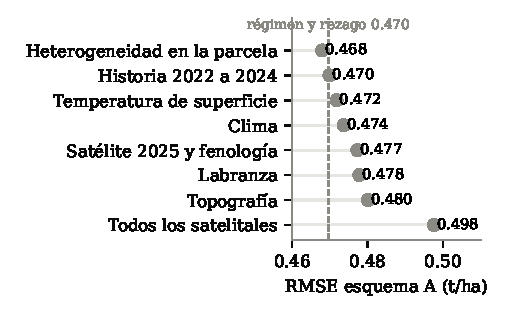
\includegraphics[width=0.60\columnwidth]{f4_bloques}
\caption{RMSE al agregar cada bloque de variables al modelo con régimen y rezago (línea punteada). Ninguno pasa la regla de decisión.}
\label{fig:bloques}
\end{figure}



Con las entradas fijas comparamos algoritmos~\cite{doc_modelo}. Los modelos de árboles de decisión~\cite{hastie2009} quedan peor que la media por
régimen. El proceso gaussiano obtiene el
menor error, aunque no supera de forma significativa a un modelo lineal con las mismas entradas (Tabla~\ref{tab:error}).



\section{Confiabilidad del error}\label{sec:confiabilidad}

\textbf{La ventaja sobre la media por régimen es pequeña y no concluyente.} Con las mismas particiones
(Tabla~\ref{tab:error}) el modelo final obtiene un RMSE de 0.458\,t/ha y la media por régimen 0.489. La prueba $t$
corregida de Nadeau y Bengio~\cite{nadeau2003}, que toma en cuenta que las particiones comparten parcelas, da $p=0.26$,
así que una diferencia de 0.03\,t/ha es común aun sin ventaja real. Frente al lineal da $p=0.38$. El $p=0.02$ de la
tabla viene de la prueba de permutación y solo indica que el rezago contiene información.

\textbf{Elegir el mejor modelo también tiene un costo.} Quedarnos con la mejor de 12 variantes favorece a la que tuvo
suerte con esas particiones~\cite{cawley2010}. La validación anidada repite la elección dentro de cada partición sin
ver las parcelas evaluadas y da 0.490, igual que la media por régimen. Por eso esperamos de 0.46 a 0.49\,t/ha en
parcelas nuevas.

\textbf{Con 59 parcelas el azar pesa más que esas diferencias.} Lo medimos con un bootstrap~\cite{efron1993}, que
sortea con reemplazo los errores observados, 37 del régimen A y 22 del B como en la partición oficial. El 90\,\% de
5000 sorteos cae entre 0.35 y 0.56\,t/ha.

\textbf{El intervalo de predicción cubre lo esperado.} El intervalo del percentil 10 al 90 debería contener el
rendimiento real en 80\,\% de los casos, y en la validación, sin usar la parcela evaluada, lo contiene en 83\,\%.

\textbf{No hay fuga de información.} Hay fuga cuando el rendimiento de una parcela se cuela en sus propias variables, y
entonces el modelo acertaría aun con los rendimientos revueltos~\cite{kaufman2012}. Revueltos dentro de cada régimen,
el RMSE nunca baja de 0.485 en 20 sorteos, contra 0.467 con los reales.


\begin{table}[!t]
\centering
\caption{Qué mide cada cifra de error (t/ha)}
\label{tab:error}
\footnotesize
\begin{tabular}{@{}l@{}r@{}}
\toprule
Qué se mide & RMSE \\
\midrule
Media por régimen, validación cruzada repetida & 0.489 \\
Más rezago, lineal (mejora en 9 de 10, $p=0.02$) & 0.470 \\
Proceso gaussiano (contra el lineal, $p=0.38$) & 0.458 \\
Elegir entre 12 variantes, validación anidada & 0.490 \\
Azar con 59 parcelas (90\,\% de 5000 sorteos)\quad & 0.35 a 0.56 \\
\bottomrule
\end{tabular}
\end{table}


\section{Preguntas guía}

Las bases del reto plantean tres preguntas guía~\cite{bases}. El modelo final no usa índices ni clima, así
que no puede ordenarlos. Para responder usamos un bosque aleatorio~\cite{breiman2001} de análisis con todas las variables y medimos cuánto
sube su RMSE al revolver los valores de cada índice (Fig.~\ref{fig:indices}).

\textbf{Índice satelital.} Sin el régimen, el índice de vegetación NDVI~\cite{tucker1979} es el más importante. Con régimen y rezago presentes, el índice de sequía NDDI~\cite{gu2007} es el mayor, con apenas
0.004\,t/ha.

\textbf{Variable climática.} En las parcelas ninguna aporta una vez conocido el régimen. A escala regional la de mayor
peso es la temperatura máxima (Tmax) de julio y agosto~\cite{verdin2020} (Sección~\ref{sec:municipal}).

\textbf{Combinación.} Régimen más rezago espacial. Conservamos el rezago porque no empeora el error, usa información local cuando la hay y pasó la regla de
decisión fijada de antemano.

\begin{figure}[!htb]
\centering
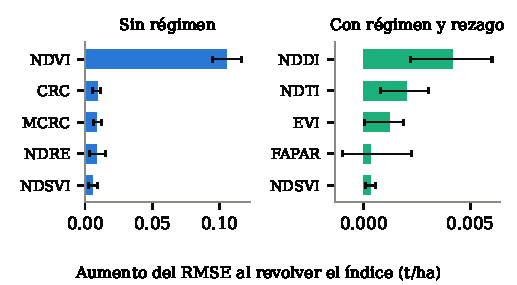
\includegraphics[width=0.60\columnwidth]{f11_indices}
\caption{Aumento del RMSE al revolver cada índice~\cite{ecuaciones} en el bosque de análisis, sin régimen (izquierda) y con régimen y
rezago (derecha). Las escalas horizontales son distintas.}
\label{fig:indices}
\end{figure}

\section{Modelo municipal con datos públicos}\label{sec:municipal}


El modelo de parcelas solo sirve donde hay parcelas con rendimiento cerca. Para estimar en toda la región usamos el
rendimiento municipal del Servicio de Información Agroalimentaria y Pesquera (SIAP)~\cite{siap} de 2003 a 2025 en
Hidalgo, México, Puebla y Tlaxcala, con 100 municipios con historia, y la Tmax de julio y agosto~\cite{verdin2020}. La unidad es el municipio,
con el promedio de sus años, porque los años de un mismo municipio no son independientes. El rendimiento esperado del
municipio $m$ es
\begin{equation}
\hat{\bar y}_m = \beta_0 + \beta_1 T_m + \hat e(\mathbf{s}_m),
\label{eq:municipal}
\end{equation}
donde $T_m$ es su Tmax y $\hat e$ un kriging de los errores de la regresión~\cite{oliver2014}, con covarianza Matérn~\cite{rasmussen2006}
ajustada en cada partición. Lejos de los datos queda solo la predicción por clima.

\textbf{Funciona en lugares sin datos.} Predecimos zonas completas sin usar municipios a menos de 50\,km~\cite{roberts2017}.
Ahí el modelo obtiene un RMSE de 0.44\,t/ha, contra 0.57 del kriging de vecinos, que no usa
clima (Fig.~\ref{fig:municipal_modelos}). El intervalo de confianza del 95\,\% de la diferencia va de $-0.18$ a $-0.09$. Cada municipio pesa según su superficie sembrada, porque FIRA opera donde hay más, y la
tendencia de los años se estima solo con el entrenamiento. Al repetir
de forma anidada la elección de la variable la ventaja baja a unos 0.07\,t/ha. Con vecinos cerca ambos empatan.

\begin{figure}[!htb]
\centering
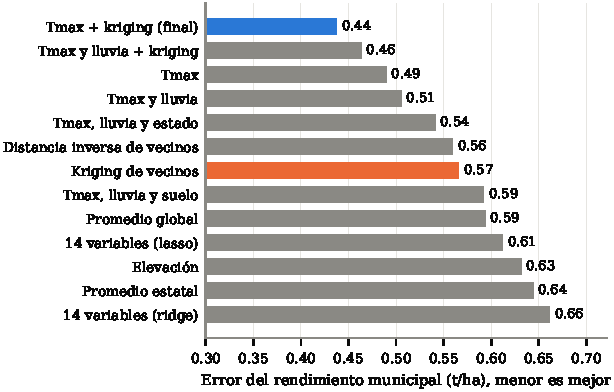
\includegraphics[width=\columnwidth]{g_modelos_simple}
\caption{Error de 13 modelos al predecir municipios sin datos del SIAP a menos de 50\,km, ponderado por superficie. En naranja el kriging de vecinos y en azul el modelo final. Lasso~\cite{tibshirani1996} y ridge~\cite{hoerl1970} usan 14 variables.}
\label{fig:municipal_modelos}
\end{figure}



\textbf{El calor de verano es la variable climática clave.} Cada grado más de Tmax se asocia con 0.79\,t/ha menos de
rendimiento (Fig.~\ref{fig:dispersion}), lo que concuerda con el daño del calor al llenado del grano~\cite{passarella2002}.
En los 9 municipios del reto la Tmax solo va de 23.3 a 23.9\,$^\circ$C. Por eso el clima no ayudó al modelo de parcelas.

\begin{figure}[!htb]
\centering
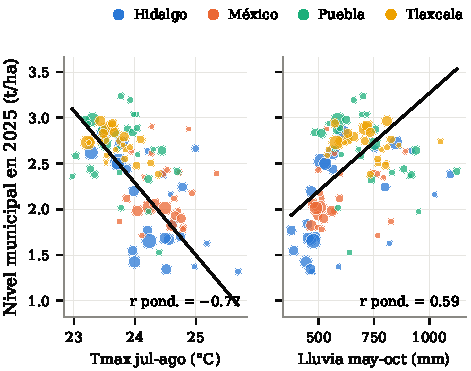
\includegraphics[width=0.60\columnwidth]{g_dispersion}
\caption{Rendimiento municipal llevado a 2025 contra la Tmax de julio y agosto y la lluvia de mayo a octubre. El tamaño del punto crece con la superficie sembrada.}
\label{fig:dispersion}
\end{figure}



\textbf{Mapa regional.} La Fig.~\ref{fig:mapas} muestra el rendimiento esperado y la probabilidad de quedar bajo
2\,t/ha. De los 486 municipios de la región mostramos 268, los que tienen la Tmax, la lluvia, la elevación y el suelo dentro del mínimo
y el máximo de los 100 municipios con SIAP~\cite{meyer2021}. La probabilidad usa los errores anuales de otras
zonas, reescalados a la variación del municipio. Sin ponderar predice 0.48 contra 0.41 observado, así que es una guía
preliminar. La confianza es alta en los 100 con SIAP, media en los de temporal a 25\,km o menos de uno de ellos y
baja en el resto, donde solo cuenta el clima.

\begin{figure}[!htb]
\centering
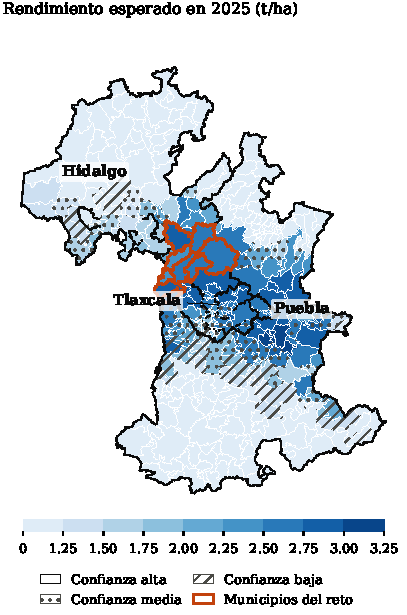
\includegraphics[width=0.60\columnwidth]{g5_mapa_a}
\caption{Rendimiento esperado en 2025. Rayado de puntos, confianza media, y de líneas, baja. En gris, ambiente fuera del rango de los datos.}
\label{fig:mapas}
\end{figure}

\begin{figure}[!htb]
\centering
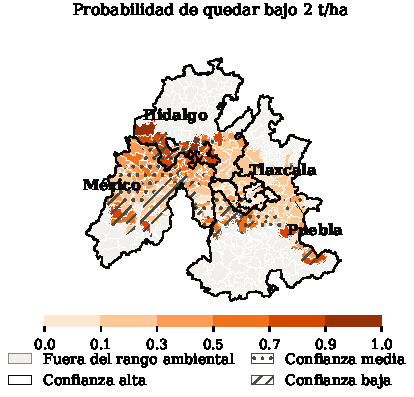
\includegraphics[width=0.60\columnwidth]{g5_mapa_b}
\caption{Probabilidad de quedar bajo 2\,t/ha en un año cualquiera. Rayado y gris como en la Fig.~\ref{fig:mapas}.}
\label{fig:mapas_prob}
\end{figure}


\section{Capa de crédito}

La probabilidad de no cubrir un umbral $u$, que puede ser el crédito o el costo total por hectárea entre el precio, es
\begin{equation}
P = q + (1-q)\,\Pr\!\left(\hat y_i + r_g < u\right),
\label{eq:credito}
\end{equation}
donde $q$ es la fracción de superficie que el municipio pierde históricamente~\cite{siap2026} y la segunda parte usa
los mismos errores de~\eqref{eq:intervalo}. Si la cosecha se pierde el ingreso es cero, por eso se suma $q$. Es una ilustración al cierre de 2025
(Sección~VIII). Antes de la siembra solo se conoce el régimen, y los $r_g$ son errores entre parcelas de 2025 que no
incluyen la variación entre años, de la que $q$ y el modelo municipal capturan una parte.

\textbf{Los parámetros salen de fuentes públicas} (Tabla~\ref{tab:credito}). El precio es el medio rural del SIAP de
2023 a 2025 en cada municipio, ponderado por la producción~\cite{siap}. El costo total y el crédito son los del paquete
de temporal 2022 de AgroCostos para la zona~\cite{agrocostos}, actualizados a 2025 con el INPC~\cite{inpc}.

\textbf{Un semáforo resume la probabilidad.} Es verde si $P<0.10$, amarillo si $0.10\le P<0.30$ y rojo si
$P\ge0.30$. La probabilidad es el resultado principal y el semáforo solo la resume, con cortes que FIRA puede mover. Con el costo total casi todas salen en rojo, porque su umbral supera casi todas las predicciones. Con el
crédito el color depende sobre todo del municipio, porque el precio, el crédito y $q$ son municipales. Las 29 parcelas
de Chignahuapan salen en amarillo y las 6 rojas son de Singuilucan.

\textbf{El error del modelo en pesos.} El error de 0.46\,t/ha por el precio de cada municipio
(Tabla~\ref{tab:credito}) da de 2,000 a 3,300\,pesos/ha, de 7 a 12\,\% del costo total y de 13 a 45\,\% del crédito. Sin
sumar $q$, 18 parcelas, todas del régimen B, tienen $\Pr(y<2.5\,\text{t/ha})>0.10$.

\begin{table}[!t]
\centering
\caption{Parámetros de la capa de crédito en las 59 parcelas}
\label{tab:credito}
\footnotesize
\begin{tabular}{@{}l@{}r@{}}
\toprule
Parámetro & Rango \\
\midrule
Precio medio rural 2023 a 2025 (pesos/t) & 4,291 a 7,224 \\
Costo total 2025 (pesos/ha) & 24,773 a 28,377 \\
Crédito más interés 2025 (pesos/ha) & 6,561 a 15,015 \\
Pérdida histórica $q$, 2003 a 2025 & 0.019 a 0.118 \\
\midrule
Verde, amarillo y rojo con el crédito & 23, 30 y 6 \\
Verde, amarillo y rojo con el costo total\quad & 0, 4 y 55 \\
\bottomrule
\end{tabular}
\end{table}

\section{Alcance y limitaciones}

\textbf{El modelo de parcelas estima al cierre de la temporada.} El rezago usa rendimientos de vecinos de la misma
temporada, que solo existen después de su cosecha. En otros municipios no se conoce el régimen, y ahí sirve el modelo
de la Sección~\ref{sec:municipal}.

\textbf{Sin vecinos la predicción es la del régimen.} De las 59 parcelas, 36 tienen al menos un vecino de entrenamiento
del mismo régimen a 400\,m o menos, 28 del A y 8 del B. Las otras 23 usan como rezago la media de su régimen y
reciben 4.54\,t/ha en el A y 3.02 en el B. Con vecinos la corrección es chica, de 4.54 a 4.58\,t/ha en 31 de las 37 A.

\textbf{El origen de los regímenes es incierto.} Según FIRA, la comercializadora reporta la mayoría de los
rendimientos y el productor el resto~\cite{preguntas}, y suponemos que cada régimen es una
fuente~\cite{doc_regimenes}, pero FIRA no dará la fuente por parcela. El SIAP de 2023 a 2025 no muestra la brecha, pues promedia 2.51\,t/ha en
los municipios A y 2.48 en los B, contra 4.51 y 3.02 en el reto, así que el B se parece más. Si el B solo se anotó distinto, la capa de crédito
castigaría a sus municipios, por eso el semáforo debe leerse junto con el régimen.

\begin{table}[!b]
\centering
\caption{Síntesis de los prompts principales}
\label{tab:ia}
\scriptsize\renewcommand{\arraystretch}{1.35}
\begin{tabular}{@{}>{\raggedright\arraybackslash}p{3.7cm}>{\raggedright\arraybackslash}p{4.25cm}@{}}
\toprule
Prompt & Resultado y uso \\
\midrule
Identificar el problema del dataset. & Diagnóstico del ruido de las etiquetas. \\
Proponer un plan de validación. & Regla de decisión fijada de antemano. \\
Auditar el código del modelo. & Rezago con la propia etiqueta, corregido. \\
Auditar de forma independiente. & Motivó el modelo municipal. \\
Investigar qué explica los regímenes. & Hipótesis de fuente mixta, no confirmada. \\
Diseñar la capa de crédito. & Capa con supuestos revisados. \\
Atender al asesor. & Auditoría sin fuga y correcciones. \\
\bottomrule
\end{tabular}
\end{table}

\section{Aportaciones y uso de inteligencia artificial}

\textbf{Vicente Josimar López Martínez}, aplicación web, levantamiento de necesidades [por confirmar], pruebas de uso
[por confirmar] y despliegue [por confirmar]. \textbf{Luis Emmanuel Ramiro Luna}, video, guion [por confirmar] y
grabación y edición [por confirmar]. \textbf{José Alán Pomares Valdés}, datos, variables, validación, modelos, capa
de crédito y redacción. \textbf{Luis Gustavo Olivares Soto}, asesor, revisión crítica de la metodología y
la redacción. Usamos Claude Code~\cite{claudecode}, de Anthropic, para programar, auditar y redactar, y verificamos cada resultado
(Tabla~\ref{tab:ia}).



% Referencias en estilo IEEE, numeradas en orden de primera cita (las genera plataforma.py).

\clearpage
% Unas líneas más para que las referencias quepan en una página.
\enlargethispage{5\baselineskip}
% Generado por plataforma.py. Estilo IEEE, en orden de primera cita.
\begin{thebibliography}{99}

\bibitem{bases}
FIRA, \emph{Reto AgroCebada 2026. Bases de participación y descripción del conjunto de datos},
  2026.

\bibitem{sader2025}
Secretaría de Agricultura y Desarrollo Rural, ``Del campo a la copa: el recorrido de la cebada,'' \emph{gob.mx}, 11 de noviembre de 2025. [En línea]. Disponible: \url{https://www.gob.mx/agricultura/articulos/del-campo-a-la-copa-el-recorrido-de-la-cebada}

\bibitem{preguntas}
FIRA, \emph{Sesiones de preguntas y respuestas del Reto AgroCebada 2026 y correos de seguimiento a los equipos participantes}, septiembre y octubre de 2026 (último correo del 14 de octubre).

\bibitem{drusch2012}
M. Drusch \emph{et al.}, ``Sentinel-2: ESA's Optical High-Resolution Mission for GMES Operational Services,'' \emph{Remote Sensing of Environment}, vol.~120, pp.~25--36, 2012.

\bibitem{frazier2021}
A.~E. Frazier y B.~L. Hemingway, ``A Technical Review of Planet Smallsat Data: Practical Considerations for Processing and Using PlanetScope Imagery,'' \emph{Remote Sensing}, vol.~13, no.~19, p.~3930, 2021.

\bibitem{funk2015}
C. Funk \emph{et al.}, ``The climate hazards infrared precipitation with stations---a new environmental record for monitoring extremes,'' \emph{Scientific Data}, vol.~2, art.~150066, 2015.

\bibitem{verdin2020}
A. Verdin \emph{et al.}, ``Development and validation of the CHIRTS-daily quasi-global high-resolution daily temperature data set,'' \emph{Scientific Data}, vol.~7, no.~1, art.~303, 2020.

\bibitem{vanklompenburg2020}
T. van Klompenburg, A. Kassahun y C. Catal, ``Crop yield prediction using machine learning: A systematic literature review,'' \emph{Computers and Electronics in Agriculture}, vol.~177, p.~105709, 2020.

\bibitem{weiss2020}
M. Weiss, F. Jacob y G. Duveiller, ``Remote sensing for agricultural applications: A meta-review,'' \emph{Remote Sensing of Environment}, vol.~236, p.~111402, 2020.

\bibitem{lobell2020}
D.~B. Lobell \emph{et al.}, ``Eyes in the Sky, Boots on the Ground: Assessing Satellite‐ and Ground‐Based Approaches to Crop Yield Measurement and Analysis,'' \emph{American Journal of Agricultural Economics}, vol.~102, no.~1, pp.~202--219, 2020.

\bibitem{agrocostos}
Fideicomisos Instituidos en Relación con la Agricultura, ``Agrocostos.'' [En línea]. Disponible: \url{https://www.fira.gob.mx/Nd/Agrocostos.jsp}. Consultado el 15 de octubre de 2026.

\bibitem{ecuaciones}
FIRA, \emph{Ecuaciones de índices satelitales. Reto AgroCebada FIRA 2026}, 2026.

\bibitem{zadoks1974}
J.~C. Zadoks, T.~T. Chang y C.~F. Konzak, ``A decimal code for the growth stages of cereals,'' \emph{Weed Research}, vol.~14, no.~6, pp.~415--421, 1974.

\bibitem{roberts2017}
D.~R. Roberts \emph{et al.}, ``Cross-validation strategies for data with temporal, spatial, hierarchical, or
phylogenetic structure,'' \emph{Ecography}, vol.~40, no.~8, pp.~913--929, 2017.

\bibitem{ploton2020}
P. Ploton \emph{et al.}, ``Spatial validation reveals poor predictive performance of large-scale ecological mapping models,'' \emph{Nature Communications}, vol.~11, no.~1, art.~4540, 2020.

\bibitem{ojala2010}
M.~Ojala y G.~C. Garriga, ``Permutation tests for studying classifier performance,'' \emph{Journal of Machine
Learning Research}, vol.~11, pp.~1833--1863, 2010.

\bibitem{tobler1970}
W.~R. Tobler, ``A computer movie simulating urban growth in the Detroit region,'' \emph{Economic Geography},
vol.~46, pp.~234--240, 1970.

\bibitem{rasmussen2006}
C.~E. Rasmussen y C.~K.~I. Williams, \emph{Gaussian Processes for Machine Learning}. Cambridge, MA, EE.~UU.: MIT
Press, 2006.

\bibitem{vovk2005}
V.~Vovk, A.~Gammerman y G.~Shafer, \emph{Algorithmic Learning in a Random World}. Nueva York, NY, EE.~UU.:
Springer, 2005.

\bibitem{lei2018}
J. Lei \emph{et al.}, ``Distribution-Free Predictive Inference for Regression,'' \emph{Journal of the American Statistical Association}, vol.~113, no.~523, pp.~1094--1111, 2018.

\bibitem{cawley2010}
G.~C. Cawley y N.~L.~C. Talbot, ``On over-fitting in model selection and subsequent selection bias in performance
evaluation,'' \emph{Journal of Machine Learning Research}, vol.~11, pp.~2079--2107, 2010.

\bibitem{varma2006}
S.~Varma y R.~Simon, ``Bias in error estimation when using cross-validation for model selection,'' \emph{BMC
Bioinformatics}, vol.~7, art.~91, 2006.

\bibitem{nadeau2003}
C.~Nadeau e Y.~Bengio, ``Inference for the generalization error,'' \emph{Machine Learning}, vol.~52, no.~3,
pp.~239--281, 2003.

\bibitem{kaufman2012}
S.~Kaufman, S.~Rosset, C.~Perlich y O.~Stitelman, ``Leakage in data mining: Formulation, detection, and
avoidance,'' \emph{ACM Transactions on Knowledge Discovery from Data}, vol.~6, no.~4, art.~15, 2012.

\bibitem{siap2026}
SIAP, ``Producción agrícola municipal, cierre 2025,'' Datos abiertos, 2026. Consultado el 4 de
  octubre de 2026. Disponible en \url{https://nube.agricultura.gob.mx/datosAbiertos/Agricola.php}

\bibitem{gu2007}
Y. Gu \emph{et al.}, ``A five‐year analysis of MODIS NDVI and NDWI for grassland drought assessment over the central Great Plains of the United States,'' \emph{Geophysical Research Letters}, vol.~34, no.~6, art.~2006GL029127, 2007.

\bibitem{jensen2017}
N. Jensen y C. Barrett, ``Agricultural Index Insurance for Development,'' \emph{Applied Economic Perspectives and Policy}, vol.~39, no.~2, pp.~199--219, 2017.

\end{thebibliography}


\end{document}
